\chapter{Introduction}
\label{cha:introduction}
FPGA(Field Programmable Gate Array) is special hardware device that allows people can design and verify their thoughts easily and quickly comparing to ASIC. To design hardware part in PL(Programmable Logic) side, it need to use development tools(e.g.Vivado) provided by FPGA's manufaction. It is reasonable, because how to convert HDL to the designs that FPGA can recognize depends on rules of its own provider. So hardware design facilitation is basicly in control of FPGA vendors. On the other hand, software designing should be much easier and more free, because we can use languages and libaries that we are familiar with. But in fact, we still rely on using SDK tools to design our software system instead. In tradition, we build a ``bare metal'' program to control our system, and sometimes, the program may includes some special libraries only provided in SDK. In software engineer's perspective, things should not be that complicated if we just want to do the simple things like, reading or writing datas to registers in PL side. So there come's some solutions to flexible the software development.  
%本章為簡易的LaTeX範本,使本文略微豐富些。由於編譯器是使用XeLaTeX,中英文可以無縫直接輸入,不需要額外繁瑣的環境設定。 Section~\ref{sec:simpletechnique1} 是撰寫文件時可以用的一些小技巧。 Section~\ref{sec:figandtable} 示範LaTeX繪製圖表的功能。

%-------------------------------------------------------------------------
% Section: 簡單範例和小技巧
%-------------------------------------------------------------------------

\section{Motivation}
\label{sec:Motivation}

 To simplify the develop flow, introducing embedded system on FPGA becomes more popular in recent years. In embedded Linux we can apply UIO driver to our custom IP in PL side and control it in user space application, just like it is a external device. However there are still some issues, that make UIO can not work correctly, the designs using AXI-Stream register with DMA controller is the one of them. With this design, we can only control DMA controller to transfer data ``to'' or ``from'' our custom IP, and this need ``root'' privileges. But giving ``root'' to a user that only want to control the custom IP is overkill. So we need to find out a soluion to this problem. 

%首先先示範一行簡單的數學式:
%\begin{equation} \label{eq:sample1}
%  y = \sum_{i=1}^{n}f(x_i),
%\end{equation}
%個人認為這比起用 Word 的方程式專業不少,在輸入上也方便得多。不過有些人可能會發現這條式子和一些常見的課本(像微積分)上的式子長得略微不同,這是因為他們額外安裝了付費的數學字型 MathTime Professional,約莫台幣三千元,可以讓 $y$ 和一些粗體希臘字母長得好看些,一些數學符號的間距也會被修正。

%不管是哪個科系,很多時候會需要把一些數據寫進論文裡。若是在論文撰寫的同時仍然有機會更動數據,那麼找出該數字出現的每個地方並一一改寫,這是一件很崩潰的事。所以小弟我的做法是把一些關鍵的數字寫在 \texttt{src/def.tex} 裡,利用 \texttt{newcommand} 去定義該數字。例如某項實驗做出來的準確度為 \expACC{}\%,那麼之後需要變動就只要改寫 \texttt{src/def.tex} 中的 \texttt{expACC} 即可。

%在編譯完一份文件,切莫忘記檢查 \texttt{.log} 檔案中是否含有 Overfull hbox 或 Underfull hbox 等訊息。前者代表存在一行文字無法左右貼齊,會有文字超出到頁邊空白處,後者則是在左右貼齊的過程中,文字間的留白過大。

%-------------------------------------------------------------------------
% Section: 圖表
%-------------------------------------------------------------------------

\section{Contribution}
\label{sec:contribution}
We propose a develop flow to use UIO to control DMA controller to communicate with AXI-Stream IP, with a little modified of UIO driver and specific format settings in device tree file. We rewrite \textbf{read()/write()} functions in UIO to send DMA transactions to DMA controller. The whole scenario is very simple and intuitive, and is not much different from original flow. The data transfering efficiency is also good, it reaches about 17mb/s with AXI-Stream FIFO. 
%表格當然可以用 Excel 匯出成 PDF 或圖檔在匯進來,但我是直接用 LaTeX 繪製,如 Table~\ref{tab:sample1}。圖也是一樣, Figure~\ref{fig:lena} 是一張影像處理常用的圖。但若是漂亮的數據圖繪製,那小弟我也是推薦使用 LaTeX 的向量繪圖功能。 Figure~\ref{fig:runtimeanalysis} 是用 PGFPlots 這個套件以存放在 \texttt{data/result.txt} 的實驗數據畫的圖,若是用 Matlab 畫得就比較快但比較醜。另外值得注意的是數據越多畫越久,上千個資料點可能會需要三秒到五秒不等的時間。

%\begin{table}
%\centering
%\begin{tabular}{clr|clr}
%  \toprule
%    \textbf{Id} & \textbf{Family} & \textbf{\#} & \textbf{Id} & \textbf{Family} & \textbf{\#} \\
%  \midrule
%  A & DroidKungFu   & 473 & K & FakePlayer      &  74 \\
%  B & DorDrae       & 420 & L & Wroba           &  74 \\
%  C & Meds          & 221 & M & Plankton        &  63 \\
%  D & Fakeguard     & 203 & N & DroidDreamLight &  52 \\
%  E & Boxer         & 202 & O & Cawitt          &  51 \\
%  F & Kmin          & 183 & P & Badao           &  46 \\
%  G & Rooter        & 117 & Q & Fake10086       &  46 \\
%  H & Boqx          & 114 & R & Cupi            &  39 \\
%  I & DroidAp       & 106 & S & Coogos          &  39 \\
%  J & DroidKungFu3  &  93 & T & DroidDream      &  39 \\
%  \bottomrule
%\end{tabular}


%\caption{Top 20 malware families in the dataset.}
%\label{tab:sample1}
%\end{table}

%\begin{figure}
%  \centering
%  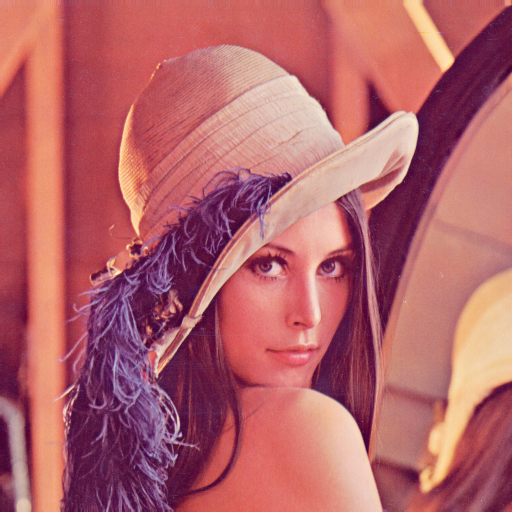
\includegraphics[scale=0.5]{images/lena.png}
%  \caption[Short caption for Lena]{Long caption for Lena.}
%  \label{fig:lena}
%\end{figure}

%\begin{figure}
%\centering
%  \begin{tikzpicture}
%    \begin{axis} [
%      xlabel={Size of classes.dex (MiB)},
%      ylabel={Time (sec)},
%      xmin=0.01,
%      xmax=144,
%      xmode=log,
%      ymin=0.01,
%      ymax=144,
%      ymode=log,
%      height=10cm,
%      width=10cm,
%      grid=major,
%      legend cell align=left,
%      legend pos=south east,
%    ]
%    
%    \addplot [color=gray,only marks,mark size=1pt] table [x=size,y=time] {data/result.txt};
%    \addplot [color=black] coordinates {(0.01,0.0471) (10,55.5648)} node[below] at (0.7, 0.7) {$O(n^{1.024})$};

%    \legend{Samples, Estimation}

%    \end{axis}
%  \end{tikzpicture}
%  \caption{Runtime analysis of Androguard.}
%  \label{fig:runtimeanalysis}
%\end{figure}

%-------------------------------------------------------------------------
% Section: 參考文獻
%-------------------------------------------------------------------------

%\section{編輯參考文獻}
%\label{sec:ref}

%LaTeX 另個方便的地方就是參考文獻,我是使用 IEEEtran 的格式,它會依照出現的次序編排。若是使用 IEEEtranS 則會以作者姓氏為依據。另外需要注意它會雞婆地把書目標題的大小寫做改動,要保持原樣就得在 \texttt{reference.bib} 的標題加括弧,像是 \cite{permissionevolution} 和 \cite{permissionevolution2} 的差別。

%-------------------------------------------------------------------------
% Section: 總結
%-------------------------------------------------------------------------

%\section{總結}
%\label{sec:summary}

%用 LaTeX 寫論文或作業很方便,但速度快慢取決於對於 LaTeX 的熟悉程度,還不熟的同學可以搜尋大家來學LaTeX \cite{latex123},以入門來說是滿不錯的,祝各位碩博士生論文順利。




